% This file was created with tikzplotlib v0.10.1.
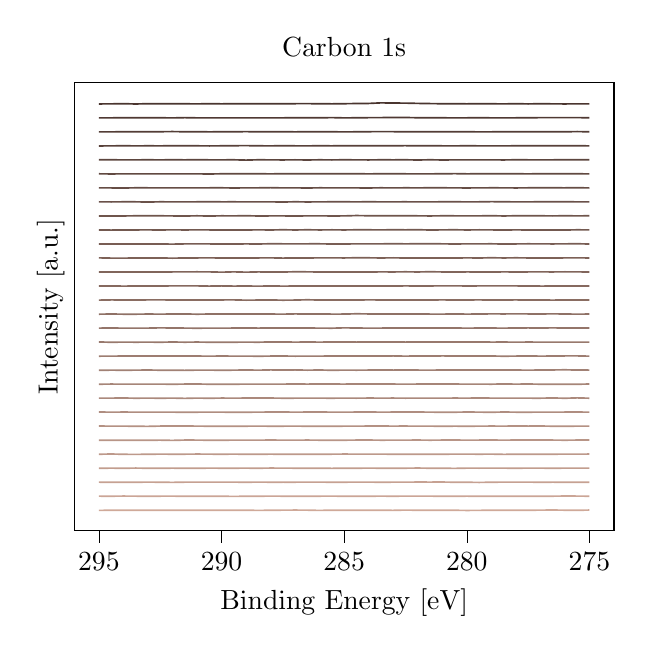
\begin{tikzpicture}

\definecolor{darkgray176}{RGB}{176,176,176}
\definecolor{darkolivegreen1027769}{RGB}{102,77,69}
\definecolor{darkolivegreen836154}{RGB}{83,61,54}
\definecolor{darkolivegreen886558}{RGB}{88,65,58}
\definecolor{darkolivegreen926962}{RGB}{92,69,62}
\definecolor{darkolivegreen977365}{RGB}{97,73,65}
\definecolor{darkslategray745347}{RGB}{74,53,47}
\definecolor{darkslategray795751}{RGB}{79,57,51}
\definecolor{dimgray1068173}{RGB}{106,81,73}
\definecolor{dimgray1118576}{RGB}{111,85,76}
\definecolor{dimgray1158980}{RGB}{115,89,80}
\definecolor{dimgray1209384}{RGB}{120,93,84}
\definecolor{dimgray1259787}{RGB}{125,97,87}
\definecolor{dimgray12910191}{RGB}{129,101,91}
\definecolor{dimgray13410595}{RGB}{134,105,95}
\definecolor{dimgray13810998}{RGB}{138,109,98}
\definecolor{gray143113102}{RGB}{143,113,102}
\definecolor{gray148117106}{RGB}{148,117,106}
\definecolor{gray152121109}{RGB}{152,121,109}
\definecolor{gray157125113}{RGB}{157,125,113}
\definecolor{gray161129117}{RGB}{161,129,117}
\definecolor{rosybrown166133120}{RGB}{166,133,120}
\definecolor{rosybrown171137124}{RGB}{171,137,124}
\definecolor{rosybrown175141128}{RGB}{175,141,128}
\definecolor{rosybrown180145131}{RGB}{180,145,131}
\definecolor{rosybrown184149135}{RGB}{184,149,135}
\definecolor{rosybrown189153139}{RGB}{189,153,139}
\definecolor{rosybrown194157142}{RGB}{194,157,142}
\definecolor{rosybrown198161146}{RGB}{198,161,146}
\definecolor{tan203165150}{RGB}{203,165,150}
\definecolor{tan207169153}{RGB}{207,169,153}

\begin{axis}[
scaled y ticks=manual:{}{\pgfmathparse{#1}},
tick align=outside,
title={Carbon 1s},
x dir=reverse,
x grid style={darkgray176},
xlabel={Binding Energy [eV]},
xmin=274, xmax=296,
xtick pos=left,
xtick style={color=black},
y grid style={darkgray176},
ylabel={Intensity [a.u.]},
ymajorticks=false,
ymin=-151524.25, ymax=8575.25,
ytick style={color=black},
yticklabels={}
]
\addplot [semithick, darkslategray745347]
table {%
295 916
294.5 943
294 1009
293.5 899
293 1006
292.5 983
292 960
291.5 970
291 934
290.5 996
290 950
289.5 987
289 979
288.5 957
288 980
287.5 972
287 1012
286.5 1020
286 995
285.5 951
285 998
284.5 1067
284 1098
283.5 1298
283 1243
282.5 1208
282 1110
281.5 1045
281 986
280.5 984
280 952
279.5 1005
279 976
278.5 927
278 1013
277.5 922
277 1002
276.5 944
276 918
275.5 954
275 940
};
\addplot [semithick, darkslategray795751]
table {%
295 -4045
294.5 -4053
294 -4000
293.5 -4028
293 -4043
292.5 -4021
292 -4072
291.5 -3982
291 -4054
290.5 -4058
290 -4058
289.5 -4055
289 -4055
288.5 -4057
288 -4045
287.5 -4051
287 -3995
286.5 -4040
286 -4032
285.5 -3967
285 -4064
284.5 -4030
284 -3984
283.5 -3961
283 -3916
282.5 -3923
282 -4012
281.5 -4032
281 -4027
280.5 -4076
280 -4046
279.5 -4013
279 -4050
278.5 -4064
278 -4044
277.5 -4035
277 -3973
276.5 -3980
276 -3979
275.5 -3968
275 -4023
};
\addplot [semithick, darkolivegreen836154]
table {%
295 -9059
294.5 -9059
294 -9016
293.5 -8995
293 -9003
292.5 -9003
292 -8949
291.5 -9019
291 -9002
290.5 -9051
290 -9024
289.5 -9017
289 -8976
288.5 -9030
288 -8998
287.5 -9007
287 -9050
286.5 -9011
286 -9044
285.5 -9020
285 -9072
284.5 -9033
284 -8994
283.5 -8958
283 -8986
282.5 -8994
282 -9035
281.5 -9026
281 -9034
280.5 -9010
280 -9023
279.5 -9055
279 -9044
278.5 -9040
278 -9034
277.5 -9012
277 -9022
276.5 -8990
276 -9031
275.5 -8953
275 -9038
};
\addplot [semithick, darkolivegreen886558]
table {%
295 -14081
294.5 -14065
294 -14005
293.5 -14069
293 -14031
292.5 -14055
292 -14005
291.5 -14034
291 -14035
290.5 -14076
290 -14037
289.5 -13997
289 -13970
288.5 -14035
288 -14055
287.5 -14012
287 -14044
286.5 -14055
286 -14023
285.5 -14048
285 -13992
284.5 -14032
284 -14028
283.5 -14001
283 -13991
282.5 -13985
282 -14003
281.5 -14001
281 -14045
280.5 -14062
280 -14016
279.5 -14051
279 -14066
278.5 -14057
278 -14034
277.5 -14028
277 -14031
276.5 -13987
276 -14012
275.5 -14014
275 -14055
};
\addplot [semithick, darkolivegreen926962]
table {%
295 -19033
294.5 -19033
294 -19053
293.5 -19062
293 -19020
292.5 -19069
292 -18997
291.5 -19052
291 -18986
290.5 -19049
290 -19051
289.5 -19030
289 -19141
288.5 -19023
288 -19057
287.5 -19081
287 -19041
286.5 -19096
286 -19032
285.5 -19076
285 -19017
284.5 -19059
284 -19077
283.5 -19028
283 -19046
282.5 -19024
282 -19105
281.5 -19021
281 -19095
280.5 -19057
280 -19048
279.5 -19074
279 -19047
278.5 -19083
278 -19019
277.5 -19044
277 -19043
276.5 -19048
276 -18986
275.5 -19023
275 -19027
};
\addplot [semithick, darkolivegreen977365]
table {%
295 -24038
294.5 -24088
294 -24049
293.5 -24050
293 -24063
292.5 -24073
292 -24060
291.5 -24045
291 -24049
290.5 -24105
290 -24029
289.5 -23999
289 -24024
288.5 -24006
288 -24061
287.5 -23997
287 -24025
286.5 -24012
286 -24006
285.5 -23998
285 -24030
284.5 -23996
284 -24063
283.5 -24005
283 -23999
282.5 -24042
282 -24051
281.5 -24044
281 -24039
280.5 -23975
280 -24046
279.5 -24031
279 -24035
278.5 -24023
278 -24007
277.5 -24062
277 -23998
276.5 -24000
276 -23997
275.5 -24029
275 -24056
};
\addplot [semithick, darkolivegreen1027769]
table {%
295 -29052
294.5 -29072
294 -29108
293.5 -29033
293 -29042
292.5 -29064
292 -29050
291.5 -29048
291 -29072
290.5 -29042
290 -29032
289.5 -29098
289 -29048
288.5 -29046
288 -28982
287.5 -29072
287 -29051
286.5 -29100
286 -29038
285.5 -29054
285 -29048
284.5 -29068
284 -29090
283.5 -29035
283 -29071
282.5 -29034
282 -29057
281.5 -29023
281 -29029
280.5 -29063
280 -29081
279.5 -29059
279 -29037
278.5 -29045
278 -29080
277.5 -29040
277 -29000
276.5 -29037
276 -29043
275.5 -29002
275 -29076
};
\addplot [semithick, dimgray1068173]
table {%
295 -34041
294.5 -34074
294 -34035
293.5 -34041
293 -34121
292.5 -34031
292 -34061
291.5 -34062
291 -34040
290.5 -33987
290 -34046
289.5 -34036
289 -34062
288.5 -34048
288 -34050
287.5 -34110
287 -34021
286.5 -34088
286 -34043
285.5 -34040
285 -34013
284.5 -34071
284 -34001
283.5 -34065
283 -34050
282.5 -34037
282 -34070
281.5 -34071
281 -34026
280.5 -34020
280 -34059
279.5 -34041
279 -33977
278.5 -34012
278 -34064
277.5 -34054
277 -34026
276.5 -33998
276 -34004
275.5 -34054
275 -34064
};
\addplot [semithick, dimgray1118576]
table {%
295 -39083
294.5 -39088
294 -39088
293.5 -39026
293 -39021
292.5 -39027
292 -39071
291.5 -39105
291 -39035
290.5 -39115
290 -39037
289.5 -39057
289 -39001
288.5 -39098
288 -39068
287.5 -39064
287 -39112
286.5 -39051
286 -39047
285.5 -39088
285 -39065
284.5 -38939
284 -39010
283.5 -39036
283 -39017
282.5 -39001
282 -39042
281.5 -39082
281 -39030
280.5 -39041
280 -39057
279.5 -39055
279 -38999
278.5 -39089
278 -39014
277.5 -39012
277 -39022
276.5 -39073
276 -39003
275.5 -39064
275 -39018
};
\addplot [semithick, dimgray1158980]
table {%
295 -44079
294.5 -44133
294 -44082
293.5 -44076
293 -44063
292.5 -44091
292 -44051
291.5 -44081
291 -44055
290.5 -44072
290 -44089
289.5 -44082
289 -44103
288.5 -44043
288 -44097
287.5 -44012
287 -44091
286.5 -44020
286 -44081
285.5 -44038
285 -44082
284.5 -44024
284 -44030
283.5 -44071
283 -44002
282.5 -44045
282 -43996
281.5 -44109
281 -44057
280.5 -44021
280 -44089
279.5 -44039
279 -44067
278.5 -44101
278 -44059
277.5 -44090
277 -44072
276.5 -44090
276 -44112
275.5 -44030
275 -44066
};
\addplot [semithick, dimgray1209384]
table {%
295 -49092
294.5 -49083
294 -49082
293.5 -49080
293 -49099
292.5 -49096
292 -49144
291.5 -49064
291 -49063
290.5 -49071
290 -49080
289.5 -49106
289 -49063
288.5 -49098
288 -49014
287.5 -49041
287 -49064
286.5 -49040
286 -49037
285.5 -49102
285 -49099
284.5 -49047
284 -49057
283.5 -49052
283 -48996
282.5 -49051
282 -49015
281.5 -49025
281 -49041
280.5 -49103
280 -49045
279.5 -49054
279 -49034
278.5 -49109
278 -49074
277.5 -49036
277 -49056
276.5 -49075
276 -49051
275.5 -49005
275 -49112
};
\addplot [semithick, dimgray1259787]
table {%
295 -54052
294.5 -54136
294 -54153
293.5 -54086
293 -54106
292.5 -54079
292 -54162
291.5 -54087
291 -54074
290.5 -54049
290 -54097
289.5 -54110
289 -54097
288.5 -54074
288 -54044
287.5 -54136
287 -54074
286.5 -54100
286 -54045
285.5 -54050
285 -54076
284.5 -54015
284 -54034
283.5 -54089
283 -54039
282.5 -54103
282 -54094
281.5 -54102
281 -54092
280.5 -54122
280 -54047
279.5 -54103
279 -54007
278.5 -54084
278 -54029
277.5 -54079
277 -54117
276.5 -54078
276 -54070
275.5 -54066
275 -54074
};
\addplot [semithick, dimgray12910191]
table {%
295 -59126
294.5 -59103
294 -59075
293.5 -59124
293 -59112
292.5 -59125
292 -59070
291.5 -59057
291 -59037
290.5 -59058
290 -59159
289.5 -59050
289 -59155
288.5 -59063
288 -59112
287.5 -59110
287 -59016
286.5 -59041
286 -59103
285.5 -59076
285 -59093
284.5 -59078
284 -59104
283.5 -59058
283 -59080
282.5 -59031
282 -59087
281.5 -59005
281 -59077
280.5 -59110
280 -59068
279.5 -59081
279 -59126
278.5 -59054
278 -59095
277.5 -59070
277 -59061
276.5 -59075
276 -59038
275.5 -59057
275 -59095
};
\addplot [semithick, dimgray13410595]
table {%
295 -64113
294.5 -64073
294 -64142
293.5 -64096
293 -64122
292.5 -64115
292 -64050
291.5 -64069
291 -64060
290.5 -64134
290 -64068
289.5 -64135
289 -64103
288.5 -64153
288 -64087
287.5 -64141
287 -64112
286.5 -64127
286 -64089
285.5 -64102
285 -64106
284.5 -64111
284 -64083
283.5 -64090
283 -64095
282.5 -64064
282 -64086
281.5 -64073
281 -64063
280.5 -64039
280 -64090
279.5 -64066
279 -64040
278.5 -64066
278 -64064
277.5 -64106
277 -64128
276.5 -64126
276 -64094
275.5 -64107
275 -64106
};
\addplot [semithick, dimgray13810998]
table {%
295 -69139
294.5 -69066
294 -69084
293.5 -69092
293 -69066
292.5 -69048
292 -69099
291.5 -69103
291 -69093
290.5 -69100
290 -69072
289.5 -69060
289 -69160
288.5 -69116
288 -69078
287.5 -69165
287 -69122
286.5 -69017
286 -69117
285.5 -69111
285 -69076
284.5 -69106
284 -69051
283.5 -69085
283 -69075
282.5 -69124
282 -69081
281.5 -69101
281 -69056
280.5 -69106
280 -69080
279.5 -69063
279 -69091
278.5 -69076
278 -69068
277.5 -69079
277 -69070
276.5 -69141
276 -69073
275.5 -69087
275 -69080
};
\addplot [semithick, gray143113102]
table {%
295 -74164
294.5 -74095
294 -74163
293.5 -74165
293 -74112
292.5 -74144
292 -74106
291.5 -74072
291 -74171
290.5 -74104
290 -74090
289.5 -74087
289 -74102
288.5 -74074
288 -74113
287.5 -74150
287 -74061
286.5 -74112
286 -74089
285.5 -74131
285 -74125
284.5 -74017
284 -74076
283.5 -74106
283 -74083
282.5 -74089
282 -74104
281.5 -74127
281 -74138
280.5 -74092
280 -74136
279.5 -74109
279 -74053
278.5 -74075
278 -74043
277.5 -74070
277 -74096
276.5 -74041
276 -74098
275.5 -74151
275 -74112
};
\addplot [semithick, gray148117106]
table {%
295 -79138
294.5 -79082
294 -79156
293.5 -79151
293 -79134
292.5 -79045
292 -79097
291.5 -79128
291 -79177
290.5 -79131
290 -79154
289.5 -79118
289 -79073
288.5 -79132
288 -79082
287.5 -79118
287 -79124
286.5 -79101
286 -79140
285.5 -79165
285 -79044
284.5 -79099
284 -79153
283.5 -79128
283 -79104
282.5 -79090
282 -79076
281.5 -79122
281 -79071
280.5 -79086
280 -79155
279.5 -79104
279 -79115
278.5 -79140
278 -79099
277.5 -79066
277 -79095
276.5 -79056
276 -79096
275.5 -79069
275 -79119
};
\addplot [semithick, gray152121109]
table {%
295 -84076
294.5 -84194
294 -84128
293.5 -84165
293 -84137
292.5 -84181
292 -84096
291.5 -84165
291 -84115
290.5 -84176
290 -84161
289.5 -84168
289 -84138
288.5 -84169
288 -84073
287.5 -84074
287 -84143
286.5 -84095
286 -84139
285.5 -84092
285 -84076
284.5 -84127
284 -84075
283.5 -84104
283 -84112
282.5 -84126
282 -84094
281.5 -84122
281 -84098
280.5 -84106
280 -84078
279.5 -84074
279 -84131
278.5 -84116
278 -84145
277.5 -84119
277 -84135
276.5 -84154
276 -84144
275.5 -84128
275 -84128
};
\addplot [semithick, gray157125113]
table {%
295 -89159
294.5 -89143
294 -89109
293.5 -89083
293 -89122
292.5 -89116
292 -89098
291.5 -89112
291 -89111
290.5 -89150
290 -89104
289.5 -89141
289 -89126
288.5 -89182
288 -89123
287.5 -89101
287 -89158
286.5 -89135
286 -89140
285.5 -89097
285 -89122
284.5 -89110
284 -89123
283.5 -89118
283 -89065
282.5 -89147
282 -89074
281.5 -89090
281 -89065
280.5 -89080
280 -89088
279.5 -89101
279 -89087
278.5 -89182
278 -89127
277.5 -89067
277 -89144
276.5 -89103
276 -89067
275.5 -89060
275 -89151
};
\addplot [semithick, gray161129117]
table {%
295 -94193
294.5 -94149
294 -94170
293.5 -94151
293 -94094
292.5 -94177
292 -94172
291.5 -94216
291 -94138
290.5 -94139
290 -94182
289.5 -94151
289 -94081
288.5 -94153
288 -94061
287.5 -94117
287 -94065
286.5 -94158
286 -94088
285.5 -94205
285 -94125
284.5 -94159
284 -94121
283.5 -94092
283 -94125
282.5 -94111
282 -94123
281.5 -94141
281 -94106
280.5 -94077
280 -94107
279.5 -94079
279 -94115
278.5 -94099
278 -94115
277.5 -94136
277 -94113
276.5 -94079
276 -94019
275.5 -94118
275 -94125
};
\addplot [semithick, rosybrown166133120]
table {%
295 -99176
294.5 -99119
294 -99150
293.5 -99125
293 -99129
292.5 -99130
292 -99189
291.5 -99120
291 -99089
290.5 -99180
290 -99193
289.5 -99164
289 -99147
288.5 -99134
288 -99128
287.5 -99136
287 -99092
286.5 -99130
286 -99085
285.5 -99105
285 -99133
284.5 -99070
284 -99120
283.5 -99097
283 -99120
282.5 -99142
282 -99121
281.5 -99084
281 -99113
280.5 -99109
280 -99149
279.5 -99125
279 -99163
278.5 -99067
278 -99146
277.5 -99090
277 -99176
276.5 -99179
276 -99209
275.5 -99192
275 -99095
};
\addplot [semithick, rosybrown171137124]
table {%
295 -104142
294.5 -104135
294 -104091
293.5 -104172
293 -104127
292.5 -104181
292 -104129
291.5 -104226
291 -104126
290.5 -104184
290 -104120
289.5 -104134
289 -104117
288.5 -104108
288 -104108
287.5 -104166
287 -104154
286.5 -104139
286 -104150
285.5 -104160
285 -104142
284.5 -104156
284 -104116
283.5 -104133
283 -104121
282.5 -104156
282 -104143
281.5 -104132
281 -104152
280.5 -104117
280 -104138
279.5 -104093
279 -104129
278.5 -104125
278 -104151
277.5 -104154
277 -104158
276.5 -104081
276 -104182
275.5 -104057
275 -104166
};
\addplot [semithick, rosybrown175141128]
table {%
295 -109090
294.5 -109152
294 -109113
293.5 -109139
293 -109124
292.5 -109142
292 -109154
291.5 -109157
291 -109159
290.5 -109124
290 -109149
289.5 -109172
289 -109180
288.5 -109131
288 -109115
287.5 -109105
287 -109138
286.5 -109115
286 -109088
285.5 -109144
285 -109142
284.5 -109117
284 -109090
283.5 -109143
283 -109117
282.5 -109109
282 -109105
281.5 -109138
281 -109188
280.5 -109172
280 -109097
279.5 -109137
279 -109193
278.5 -109094
278 -109156
277.5 -109160
277 -109145
276.5 -109137
276 -109122
275.5 -109116
275 -109131
};
\addplot [semithick, rosybrown180145131]
table {%
295 -114110
294.5 -114136
294 -114134
293.5 -114188
293 -114220
292.5 -114122
292 -114116
291.5 -114110
291 -114127
290.5 -114178
290 -114162
289.5 -114156
289 -114158
288.5 -114131
288 -114165
287.5 -114157
287 -114129
286.5 -114179
286 -114204
285.5 -114182
285 -114150
284.5 -114140
284 -114113
283.5 -114117
283 -114125
282.5 -114119
282 -114137
281.5 -114140
281 -114188
280.5 -114149
280 -114171
279.5 -114146
279 -114115
278.5 -114139
278 -114089
277.5 -114124
277 -114091
276.5 -114175
276 -114182
275.5 -114146
275 -114123
};
\addplot [semithick, rosybrown184149135]
table {%
295 -119171
294.5 -119166
294 -119164
293.5 -119158
293 -119179
292.5 -119148
292 -119227
291.5 -119117
291 -119123
290.5 -119184
290 -119183
289.5 -119135
289 -119137
288.5 -119149
288 -119100
287.5 -119146
287 -119151
286.5 -119114
286 -119159
285.5 -119199
285 -119167
284.5 -119117
284 -119103
283.5 -119160
283 -119142
282.5 -119136
282 -119109
281.5 -119160
281 -119117
280.5 -119094
280 -119152
279.5 -119122
279 -119095
278.5 -119147
278 -119102
277.5 -119122
277 -119077
276.5 -119120
276 -119168
275.5 -119113
275 -119118
};
\addplot [semithick, rosybrown189153139]
table {%
295 -124179
294.5 -124093
294 -124198
293.5 -124234
293 -124178
292.5 -124141
292 -124161
291.5 -124156
291 -124115
290.5 -124138
290 -124192
289.5 -124126
289 -124203
288.5 -124199
288 -124140
287.5 -124203
287 -124194
286.5 -124178
286 -124193
285.5 -124153
285 -124115
284.5 -124135
284 -124147
283.5 -124134
283 -124175
282.5 -124188
282 -124186
281.5 -124175
281 -124172
280.5 -124139
280 -124132
279.5 -124164
279 -124133
278.5 -124218
278 -124180
277.5 -124170
277 -124171
276.5 -124162
276 -124141
275.5 -124140
275 -124117
};
\addplot [semithick, rosybrown194157142]
table {%
295 -129202
294.5 -129138
294 -129195
293.5 -129117
293 -129187
292.5 -129193
292 -129146
291.5 -129193
291 -129189
290.5 -129139
290 -129159
289.5 -129161
289 -129143
288.5 -129178
288 -129114
287.5 -129137
287 -129157
286.5 -129172
286 -129153
285.5 -129215
285 -129153
284.5 -129170
284 -129134
283.5 -129167
283 -129176
282.5 -129160
282 -129107
281.5 -129174
281 -129173
280.5 -129224
280 -129145
279.5 -129153
279 -129138
278.5 -129140
278 -129188
277.5 -129124
277 -129136
276.5 -129186
276 -129139
275.5 -129144
275 -129138
};
\addplot [semithick, rosybrown198161146]
table {%
295 -134150
294.5 -134179
294 -134192
293.5 -134187
293 -134126
292.5 -134174
292 -134220
291.5 -134150
291 -134150
290.5 -134124
290 -134141
289.5 -134137
289 -134181
288.5 -134123
288 -134165
287.5 -134152
287 -134154
286.5 -134125
286 -134140
285.5 -134165
285 -134164
284.5 -134121
284 -134127
283.5 -134182
283 -134145
282.5 -134151
282 -134109
281.5 -134124
281 -134104
280.5 -134181
280 -134178
279.5 -134244
279 -134172
278.5 -134136
278 -134124
277.5 -134143
277 -134165
276.5 -134151
276 -134163
275.5 -134161
275 -134199
};
\addplot [semithick, tan203165150]
table {%
295 -139148
294.5 -139170
294 -139115
293.5 -139150
293 -139172
292.5 -139152
292 -139145
291.5 -139174
291 -139164
290.5 -139171
290 -139165
289.5 -139239
289 -139169
288.5 -139170
288 -139134
287.5 -139156
287 -139203
286.5 -139165
286 -139155
285.5 -139128
285 -139185
284.5 -139190
284 -139177
283.5 -139134
283 -139175
282.5 -139127
282 -139147
281.5 -139145
281 -139172
280.5 -139189
280 -139148
279.5 -139181
279 -139190
278.5 -139185
278 -139154
277.5 -139155
277 -139200
276.5 -139157
276 -139102
275.5 -139122
275 -139172
};
\addplot [semithick, tan207169153]
table {%
295 -144229
294.5 -144177
294 -144152
293.5 -144179
293 -144175
292.5 -144188
292 -144179
291.5 -144169
291 -144199
290.5 -144205
290 -144195
289.5 -144163
289 -144152
288.5 -144238
288 -144173
287.5 -144147
287 -144113
286.5 -144148
286 -144234
285.5 -144151
285 -144208
284.5 -144166
284 -144157
283.5 -144192
283 -144211
282.5 -144122
282 -144177
281.5 -144203
281 -144162
280.5 -144186
280 -144247
279.5 -144217
279 -144170
278.5 -144169
278 -144162
277.5 -144173
277 -144140
276.5 -144091
276 -144159
275.5 -144208
275 -144109
};
\end{axis}

\end{tikzpicture}
